\documentclass[a4paper]{article}
\usepackage[utf8]{inputenc}
\usepackage[polish]{babel}
\usepackage{polski}
%\usepackage{indentfirst}
%\usepackage{default}
%\usepackage{graphicx}
%\usepackage{inconsolata}
\usepackage{geometry}
\usepackage{array}
\usepackage{enumerate}
\usepackage{enumitem}
\usepackage{parskip}
\setlength{\parskip}{1ex}
\usepackage[T1]{fontenc}
\usepackage{color}
\definecolor{bluekeywords}{rgb}{0.13,0.13,1}
\definecolor{greencomments}{rgb}{0,0.5,0}
\definecolor{redstrings}{rgb}{0.9,0,0}

\begin{document}

\begin{titlepage}
    \begin{center}
        \bfseries
        \huge Politechnika Wrocławska
        \vskip.2in
        \textsc{\LARGE Wydział Elektroniki}
        \vskip.2in
        \Large Wizualizacja Danych Sensorycznych
        \vskip1.5in
        \emph{\huge Wizualizacja rozkładu ciśnienia cieczy na podstawie symulacji komputerowej}
    \end{center}

    \vskip1.4in

    \begin{minipage}{.50\textwidth}
        \begin{flushleft}
            \bfseries\large Prowadzący:\par \emph{Dr inż. Bogdan Kreczmer}
        \end{flushleft}
    \end{minipage}
    %\hskip.4\textwidth
    \begin{minipage}{.45\textwidth}
        \begin{flushright}
            \bfseries\large Studenci:\par \emph{ Adam Balawender \\ Krzysztof Kwieciński }
        \end{flushright}
    \end{minipage}

    \vskip1.3in

    \centering
    \bfseries
	\Large Semestr letni 2014/2015


\end{titlepage}

\section{Opis projektu}
\subsection{Opis szczegółowy}
Zgodnie z tematem projektu zajmiemy się komputerową symulacją ruchu cieczy oraz wizualizacją rozkładu ciśnienia w zbiorniku z płynem.
Symulacja będzie obejmowała ruch cieczy w przekroju 2D wybranego naczynia.  Umożliwione będzie "wlewanie" płynu. Ciecz zostanie przedstawiona jako zbiór cząsteczek. Postaramy się, żeby jej zachowanie było możliwie zbliżone do rzeczywistego, dlatego też zrealizowane zostanie falowanie płynu.
Dodatkowo obserwowane będzie ciśnienie cieczy i zostanie ono zwizualizowane.

[TODO] Rozszerzyc opis projektu.

\subsection{Cele}
Cele projektu są następujące:
\begin{itemize}
  \item symulacja zachowania cieczy jako zbioru oddziaływujących ze sobą cząsteczek,
  \item modelowanie właściwości fizycznych wody (gęstość i lepkość),
  \item wizualizacja rozkładu ciśnień w zbiorniku.
\end{itemize}


[TODO] Uszczegolowic opis przewidywanych efektow koncowych.


[TODO] W przypadku aplikacji nalezy wymienic (w punktach) najistotniejsze funkcjonalnosci.

\section{Plan pracy}
\subsection{Harmonogram}

[TODO] Daty, tygodnie. Dokladnosc do jedego tyg. lub wieksza!

\begin{enumerate}[label=Z\arabic*{.}]
  \item Opis projektu
  \item Zapoznanie się z biblioteką Qt
  \item Zapoznanie się z metodą SPH (Smoothed Particle Hydrodynamics)
  \item Ustalenie struktur danych
  \item Implementacja klas zbiornika oraz cząsteczek cieczy 
  \item Implementacja metod uaktualniania położenia cząsteczek
  \item Analiza błędów programistycznych
  \item Poprawianie błędów
  \item Wizualizacja ciśnienia cieczy
  \item Weryfikacja projektu z założeniami
  \item Odpowiednie modyfikacje programu
  \item Napisanie raportu końcowego
\end{enumerate}

\subsection{Kamienie milowe}
\begin{enumerate}[label=K\arabic*{.}]
  \item Przeanalizowanie artykułów na temat SPH i zapoznanie się z tą metodą
  \item Zaimplementowanie struktur danych, modelu cieczy i relacji między cząsteczkami
  \item Wizualizacja symulowanego stanu cieczy
  \item Wizualizacja ciśnienia w poszczególnych punktach zbiornika
  \item Skończona dokumentacja
\end{enumerate}

\subsection{Diagram Gantta}
\begin{figure}[h] % rysunek pływający (początek) z deklaracją 
                  % umieszczenia go na górze strony (opcja h)
  \begin{center}  % deklaracja o wycentrowaniu importowanego wykresu
    %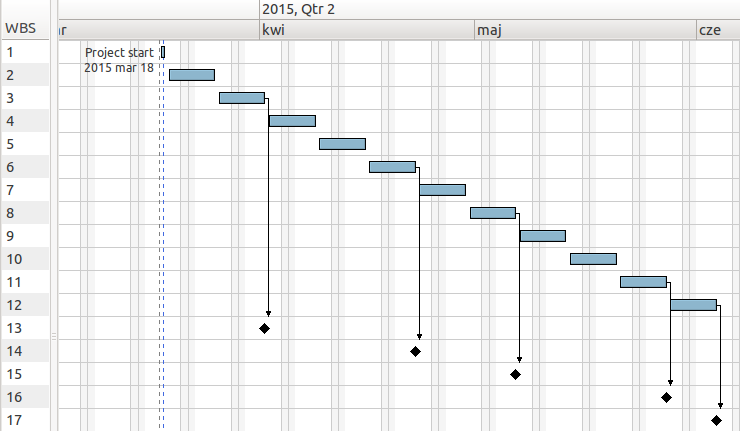
\includegraphics[width=\textwidth]{./gantt/gantt.png} % import wykresu
  \end{center}
  \caption{Wykres Gantta}
  \label{fig:gantt} % etykieta rysunku
\end{figure}       % koniec rysunku

\end{document}
